\section*{Adding Files}
After unzipping the exported calendar folder the remaining calendar file should be added to the root directory of the programs folder. The file will typically have a default name of \textbf{\textit{Calendar Name\_somestringoflettersandnumbers}}, this should be changed to a name that contains \textbf{NO SPACES}. The program will not be able to find the calendar files if their names contain spaces. Below is an example of an ideal naming convention for the file.

\begin{center}
   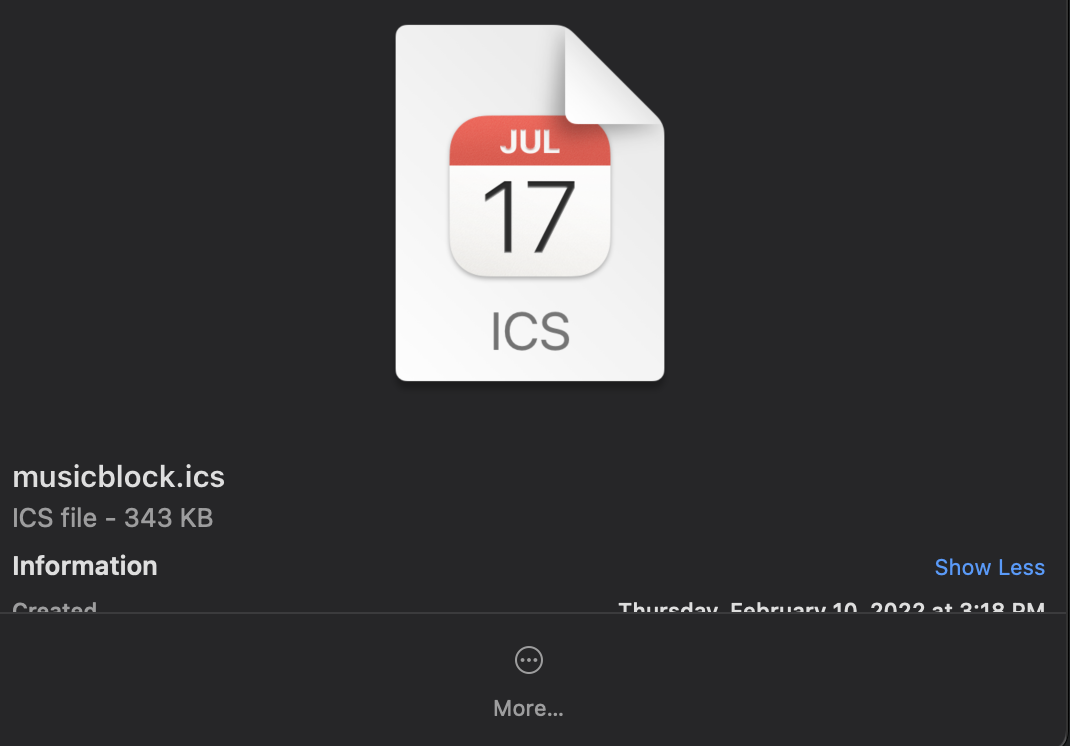
\includegraphics[width=100mm]{images/file.png} 
\end{center}